\documentclass{article}
\usepackage[polish]{babel}
\usepackage[a4paper, margin=2cm]{geometry}
\usepackage{graphicx}
\usepackage{polski}
\usepackage[utf8]{inputenc}
\usepackage{dirtytalk}
\usepackage{lettrine}
\usepackage{xcolor}
\usepackage[nodayofweek]{datetime}
\renewcommand{\familydefault}{\sfdefault}

\usepackage[autocite=superscript]{biblatex}
\addbibresource{bibliography.bib}

\title{Wspinaczka sportowa w Polsce: stosowane skale wyceny trudności tras oraz popularne rejony skałkowe}
\author{Marcin Młynarczyk}
\newdate{date}{19}{6}{2020}
\date{\displaydate{date}}
\definecolor{blue}{cmyk}{.6,.28,0,.04}

\usepackage{sectsty}
\chapterfont{\color{blue}}
\sectionfont{\color{blue}}
\subsectionfont{\color{blue}}
\subsubsectionfont{\color{blue}}

\addto\captionspolish{
  \renewcommand{\contentsname}%
    {\color{blue}Spis treści}%
}

\begin{document}

\maketitle
\tableofcontents

\bigskip

\begin{figure}[!htbp]
	\begin{center}
		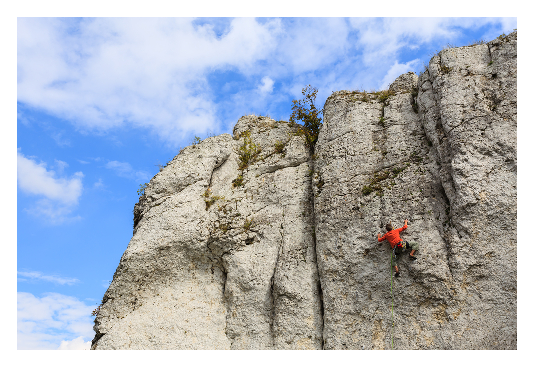
\includegraphics[width=0.9\linewidth]{images/wspin-jura.eps}
	\end{center}
	\caption{Wspinanie w skałach Jury Krakowsko-Częstochowskiej \cite{jura-intro}}
	\label{}
\end{figure}

\section{Wstęp}
%\lettrine[lines=2]{}{}

\section{Stosowane skale wyceny trudności tras sportowych w Polsce}
\lettrine[lines=2]{W}{} kulturze wspinaczkowej problem wyceny tras wydaje się być sprawą dość kontrowersyjną. W końcu, jak miał rzekomo powiedzieć Alex Lowe: \say{Najlepszym wspinaczem jest ten, kto czerpie z tego najwięcej radości} \cite{alex-lowe}. Niemniej jednak, jak w każdym sporcie i w ludzkiej naturze ogólnie, potrzeba wymierności rezultatów, czy też kategoryzacji i porównania z innymi, lub też samym sobą na przestrzeni czasu, wydaje się wygrywać. Poza tym, dopóki \say{cyfra} nie przysłania nam owej radości płynącej ze wspinania, może ona okazać się bardzo pomocna w wyborze potencjalnych projektów, czy też rywalizacji sportowej. 

Istnieje spora ilość skal wyceny tras we wspinaczce. Owa dywersyfikacja częściowo wydaje się być spowodowana istnieniem wielu odmian wspinaczki, ale również krajami w jakich owe skale są stosowane. Kraj ma bowiem wpływ na rodzaj skał i na lokalne warunki wspinaczkowe - czynniki, które są częściowo odpowiedzialne za trudność jednoznacznego porównania różnych skal wspinaczkowych, o którym trochę więcej w sekcji \ref{porownanie}. Stąd też, skale wspinaczkowe mają z reguły charakter lokalny, a ich zadaniem wydaje się być umożliwienie wspinaczom danego rejonu doboru tras na podstawie swoich poprzednich przejść. Warto tutaj nadmienić, że próby standaryzacji i globalizacji skal wspinaczkowych jak najbardziej istnieją. Opiszę w tej pracy dwie najpopularniejsze skale wyceny wspinaczkowych tras sportowych w Polsce - skalę Kurtyki spotykaną m.in. w skałach Jury Krakowsko-Częstochowskiej, oraz skalę saksońską, którą możemy spotkać w Górach Stołowych. Ponadto, wspomnę o skali francuskiej i skali \textit{UIAA}.

\subsection{Skala Kurtyki}
\label{skala-kurtyki}
Wojtek Kurtyka (rysunek \ref{kurtyka}) jest jednym z najwybitniejszych wspinaczy polskich w historii. Jednym z jego licznych dokonań było zaproponowanie w 1981 roku skali, która później przyjęła się przybierając za nazwę Jego nazwisko. Czasem nazywana jest również skalą krakowską \cite{wiki-skale}. Aby wytłumaczyć jej obecną postać, należy cofnąć się do czasów jej powstania i po krótce przedstawić skalę \textit{UIAA}. Jej nazwa jest skrótem nazwy organizacji \textit{Union Internationale des Associations d'Alpinisme}. Owa organizacja chciała wypromować ową skalę w latach 70-tych XX wieku jako uniwersalną skalę wspinaczkową dla wszystkich regionów. Jak okazało się z perspektywy lat, nie udało się to zbytnio, skala ta przyjęła się jednak przy wycenianiu dróg górskich i tam też jest najbardziej popularna. Początkowo, skala ta składała się z rzymskich cyfr od I do VI i zawierała plusy oraz minusy, aby zapewnić większą swobodę. Ponadto, jest to skala otwarta, tzn. bez górnego ograniczenia wyceny trudności. Innymi słowy, w miarę pojawiania się coraz trudniejszych tras, skala rozszerza się o kolejne stopnie razem z nimi \cite{uiaa-skala}\cite{skalnik-skale}. Skala Kurtyki miała być eleganckim rozszerzeniem skali \textit{UIAA}. Również jest to skala otwarta i do wyceny VI+ jest tożsama ze skalą proponowaną przez \textit{UIAA}. Kolejne poziomy trudności tworzone są poprzez dodanie kropki i cyfry arabskiej, następujących po rzymskim \textit{VI}. W skali dopuszcza się istnienie plusów (minusów brak), oraz stopni łamanych, np. VI.3+/VI.4 \cite{drytooling-skale}. Obecnie, najwyższą wyceną w skali Kurtyki jest VI.8. Pierwszą trasą o tej wycenie było \textit{Pandemonum} na Gołębniku - trasę tę poprowadził Rafał Moucki w 2001 roku \cite{VI8}.

\begin{figure}[!htbp]
	\begin{center}
		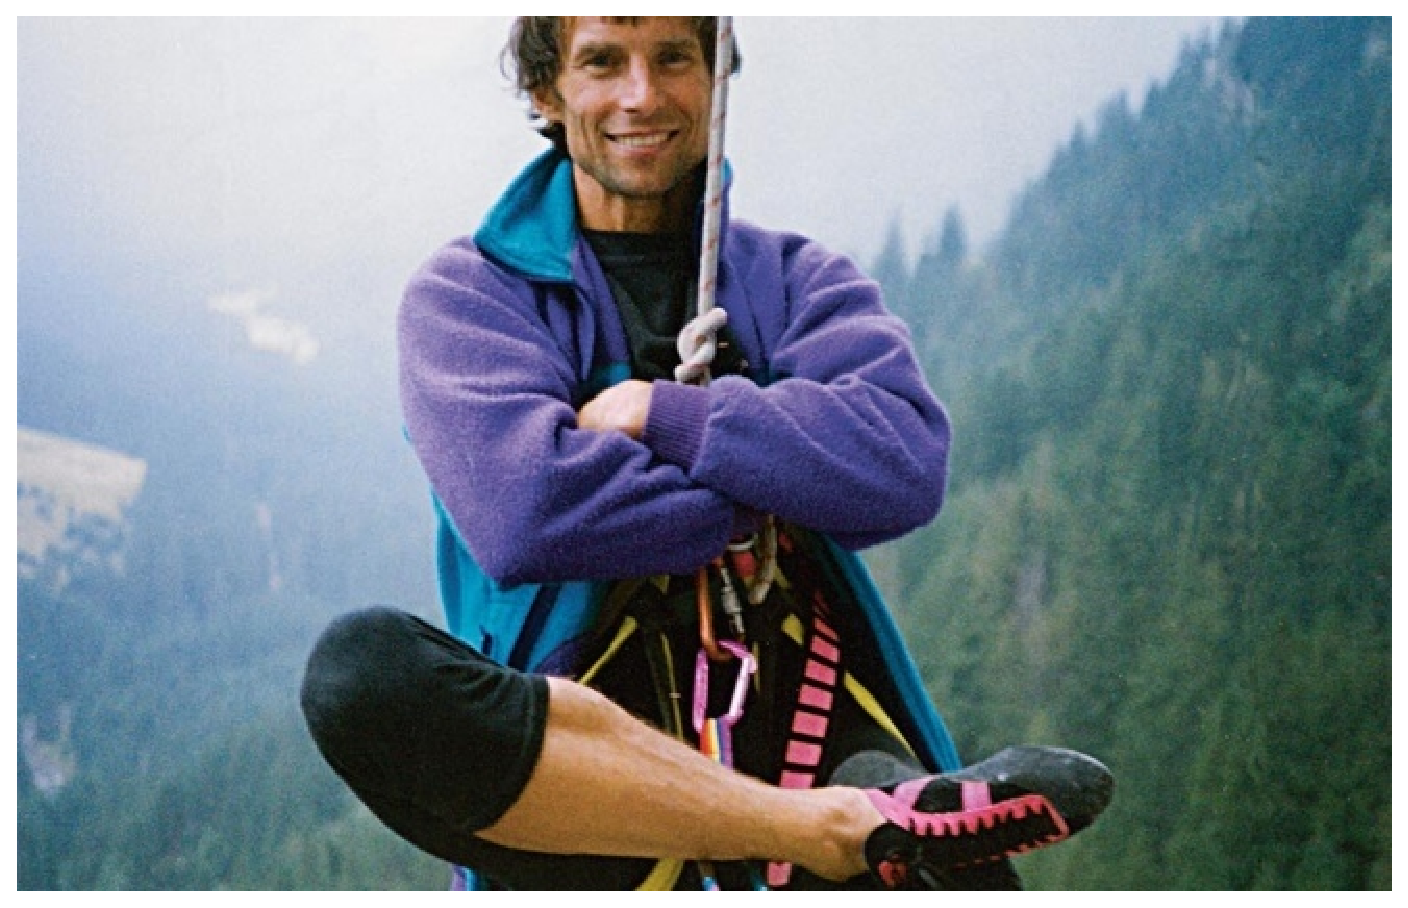
\includegraphics[width=0.9\linewidth]{images/kurtyka.eps}
	\end{center}
	\caption{Wojciech Kurtyka w Tatrach Zachodnich, droga Łamaniec na Raptawickiej Turni, lata 90. XX w. (fot. ze zbiorów Wojciecha Kurtyki) \cite{tyg-powszechni-kurtyka}}
	\label{kurtyka}
\end{figure}

\subsection{Skala saksońska}
Skala saksońska, inaczej zwana frankońską \cite{skalnik-skale} lub saską \cite{drytooling-skale}, odnosi się do wyceny tras wspinaczkowych w skałach piaskowcowych Europy Środkowej. Powstała pod koniec XIX wieku, a za jej autora uznaje się Oscara Schustera. Jej nazwa pochodzi od rejonu Szwajcarii, z którego pochodzili pionierzy tej skali. Oprócz wyceny trudności wspinaczki, składającej się z rzymskiej cyfry, określa się tutaj również wycenę trudności skoków pomiędzy skałami, które często wymagane są w trakcie wspinaczki po piaskowcu. Jak większość współczesnych skal, jest to skala otwarta, termin wyjaśniony przy wprowadzaniu skali Kurtyki (\ref{skala-kurtyki}). Od stopnia VII wyróżnia się również trzy podstopnie, które oznacza się literami a, b lub c \cite{climb-skale}. Obecnie najwyższym stopniem jest XIIb \cite{skalnik-skale}.

\subsection{Próba porównania skal}
\label{porownanie}
Na rysunku \ref{comparison} można znaleźć propozycję porównania wybranych skal wspinaczkowych, która znalazła się na blogu sklepu Skalnik \cite{skalnik-skale}. Trzy z pięciu obecnych tam skal zostało w tej pracy wspomnianych, mianowicie skala \textit{UIAA}, Kurtyki i saksońska. Szczególnie warto krótko tutaj wspomnieć o skali francuskiej, która nie została opisana wcześniej, jako że raczej nie występuje w polskich skałkach. Dominuje ona jednak w większości skalnych rejonów Europy \cite{8a-skale}. Zdaniem Piotra Czmocha \cite{8a-skale} i Maćka Smolnika \cite{weld-skale} niewykluczone, że niedługo i w Polsce skala francuska zacznie się zadomawiać. Ma to być spowodowane potrzebą łatwiejszego porównywania wspinaczkowych umiejętności, potrzebą która nabiera coraz większego znaczenia w miarę wzrostu ilości wyjazdów polskich wspinaczy do rejonów skalnych w innych krajach Europy. Dodatkowo, może się do tego przyczyniać aktywniejszy udział polskiej sceny wspinaczkowej w międzynarodowej społeczności. Postać skali francuskiej możemy wyczytać z rysunku \ref{comparison}. Skala składa się z arabskiej cyfry, a od stopnia 5 wprowadza się podstopnie reprezentowane poprzez literki a, b lub c. Ponadto, możemy tutaj spotkać plusy, które pozwalają na wskazanie dodatkowej trudności według danego stopnia, a skala jest oczywiście skalą otwartą.

\begin{figure}[!htbp]
	\begin{center}
		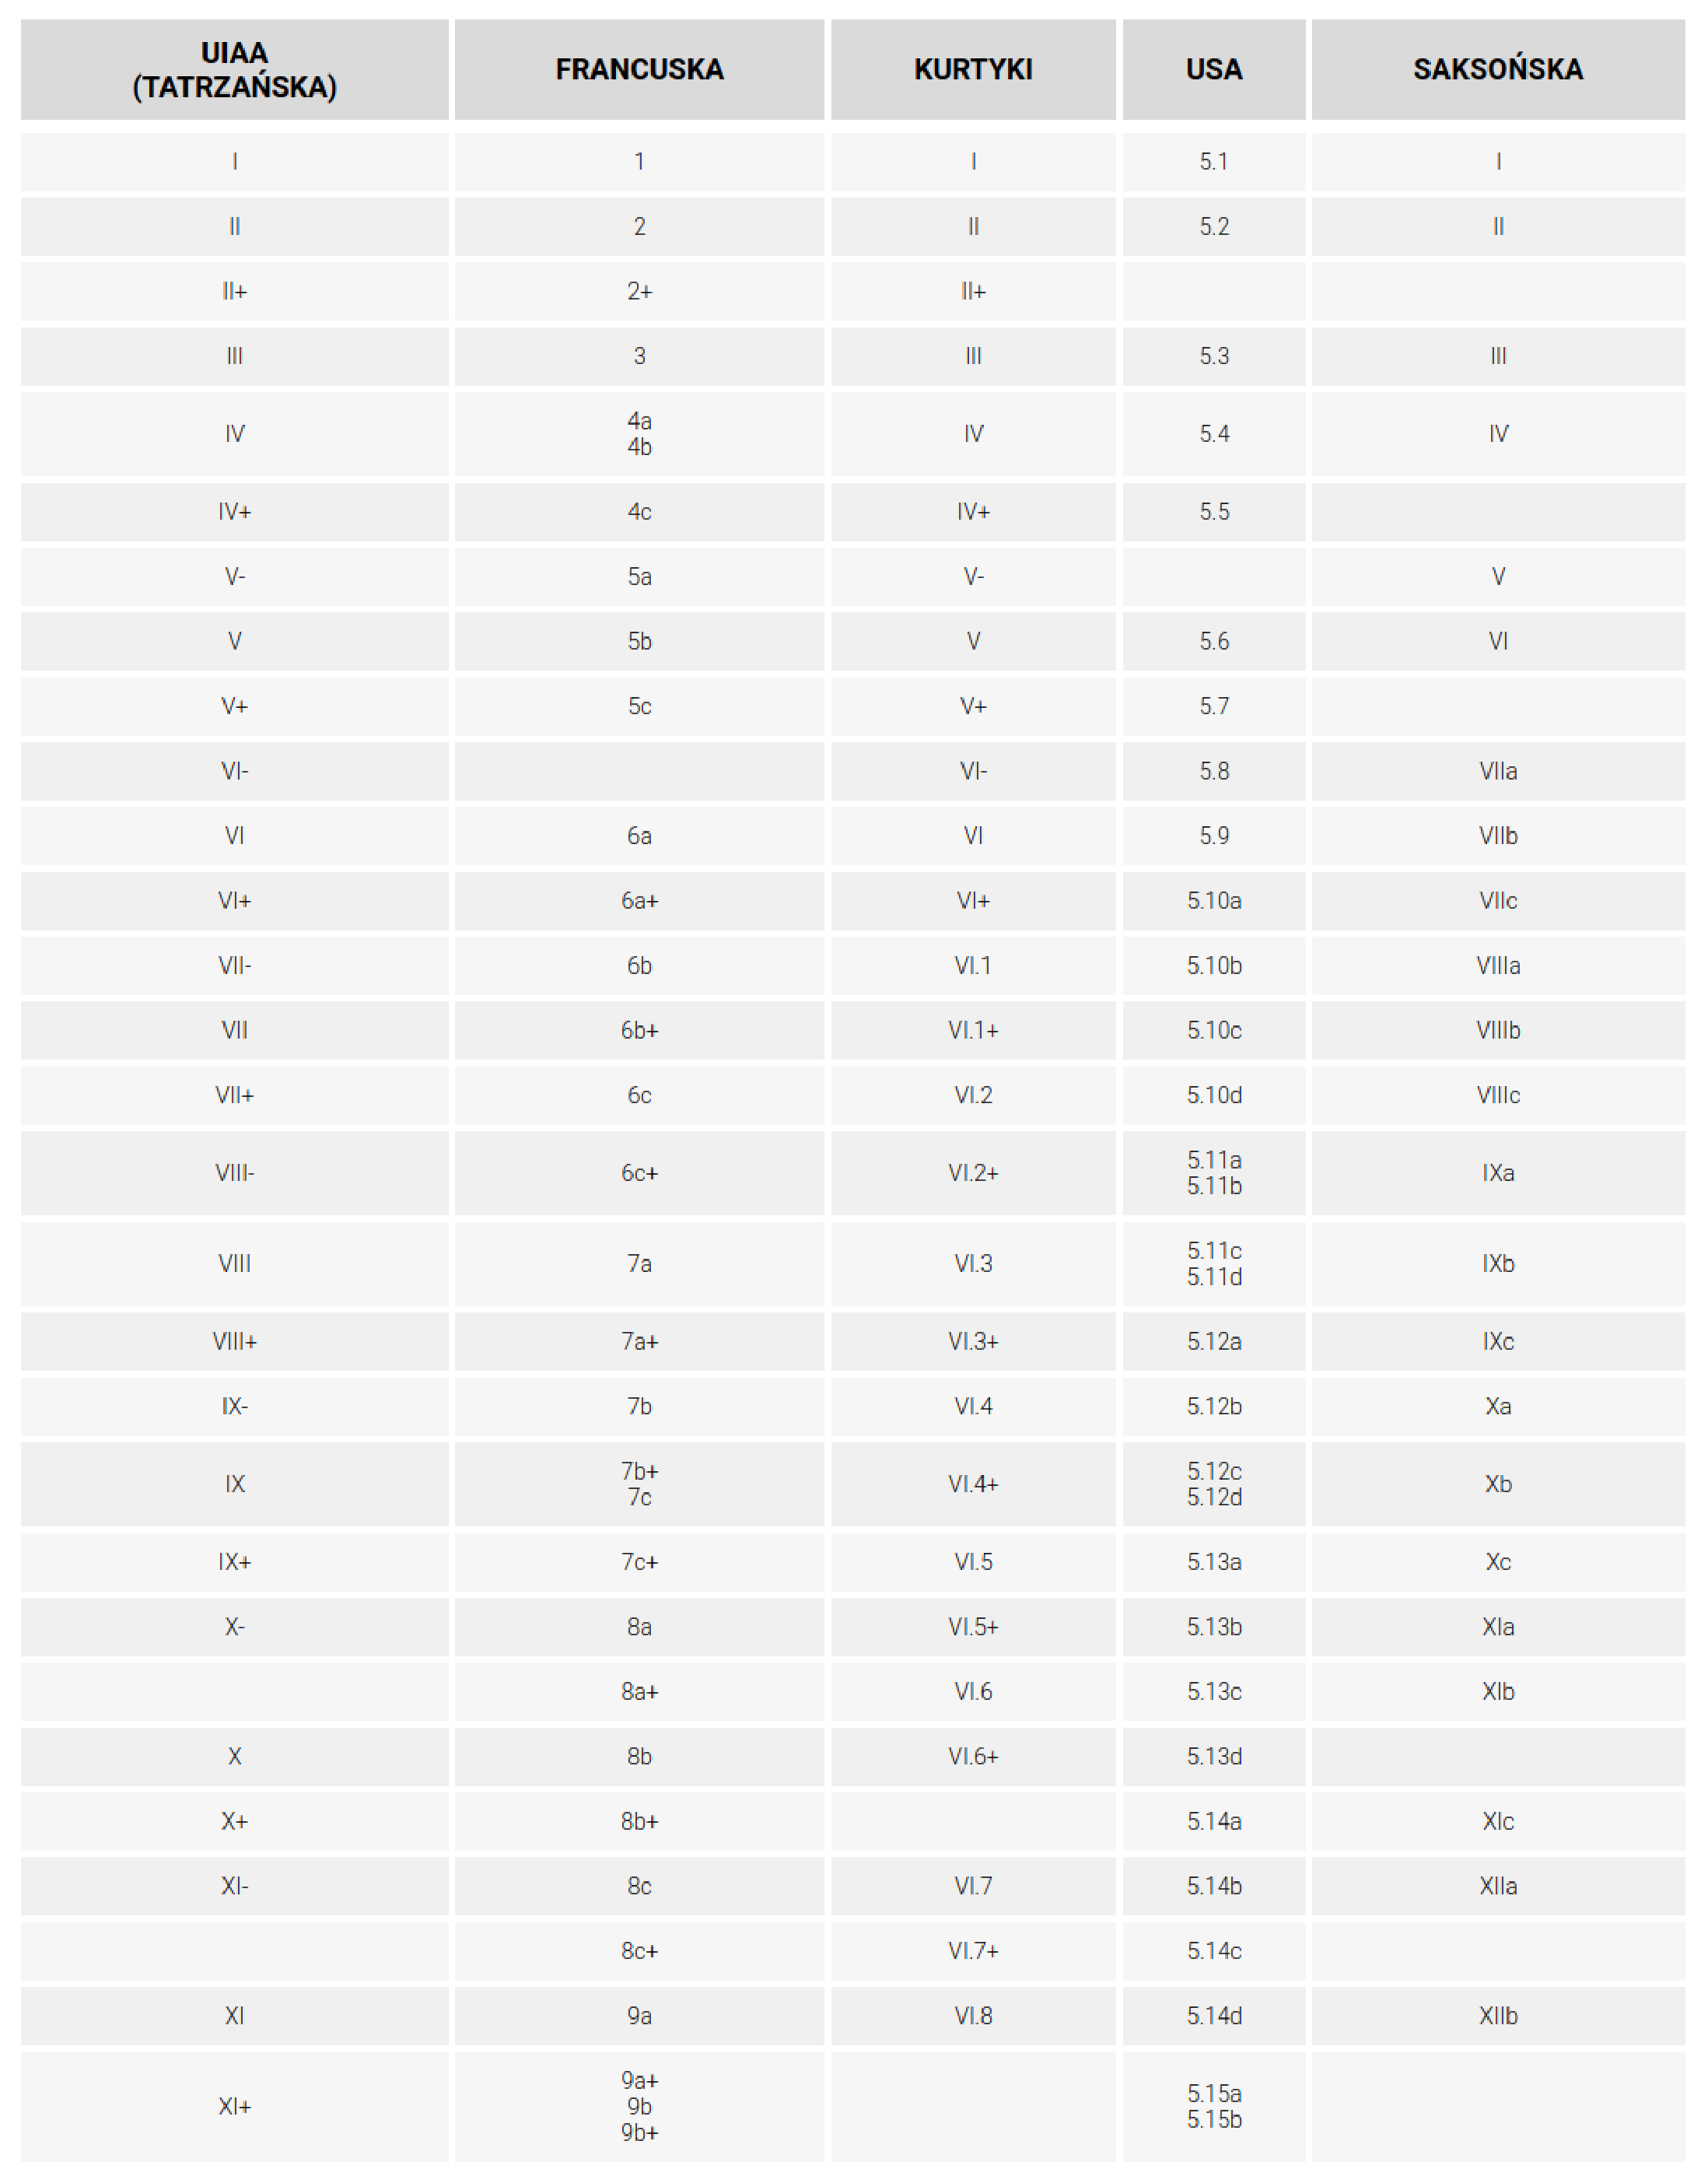
\includegraphics[width=\linewidth]{images/comparison.eps}
	\end{center}
	\caption{Porównanie wybranych skal wspinaczkowych (tabelka z portalu Skalnik)\cite{skalnik-skale}}
	\label{comparison}
\end{figure}

W swoim artykule \cite{weld-skale}, Maciek Smolnik stwierdza, że porównywanie skal ma jedynie charakter orientacyjny. Tak komentuje swoje stanowsiko: \say{Dlaczego? Dlatego że, każda wycena jest subiektywna i zależna od ogromnej liczby czynników. Ponadto, każda ze wspomnianych skal posiada różną ilość stopni trudności, co nie pozwala bezpośrednio poruszać się między każdą z nich. W wypadku wspomnianej tabeli największe zaufanie możemy mieć przy przeliczaniu trudności o wycenie 6b, 6c, 7a, 7c, reszta jest mniej lub bardziej orientacyjna. Za każdym razem pamiętajmy jednak o subiektywności wycen. Przeliczanie trudności wspinaczkowych jest czysto teoretyczne i nigdy nie będzie zero-jedynkowe. Po prostu gdy zrobimy VI.4+ to zrobiliśmy VI.4+, a gdy IX to po prostu  IX.  I chyba co najważniejsze: \say{Wspinajmy się dla przyjemności, a nie cyfry.}}. Obserwację, że porównywanie skal staje się coraz trudniejsze i potencjalnie błędne wraz ze wzrostem trudności, szczególnie na bardzo wysokim poziomie, zdaje się również podzielać Piotr Czmoch \cite{8a-skale}.

\section{Popularne rejony skałkowe w Polsce}
\lettrine[lines=2]{W}{} tej części pracy przedstawię kilka rejonów skałkowych w Polsce - począwszy od najpopularniejszej Jury, po mniej znane - Sokoliki i Góry Stołowe.

\subsection{Jura Krakowsko-Częstochowska}
Bez wątpienia jest to najczęściej odwiedzany rejon skałkowy w Polsce. Jednym z powodów owej popularności może być liczność dostępnych skał - jest to bowiem największe skupisko skał wapiennych w naszym kraju. Jura jest wyżyną rozciągającą się pomiędzy Krakowem, a Częstochową. Ze względu na swoją wielkość rejon ten jest z reguły dzielony na część północną, środkową i południową. Na Jurze trasy wyceniane według skali Kurtyki, o której wcześniej już tutaj pisano. Według statystyk na stronie Portalu Górskiego \cite{topo-jura}, na Jurze wytyczono prawie 8900 tras. Największy wybór tras znajdziemy tutaj o wycenie VI.1+ - aż 772 trasy \cite{topo-jura}, ale również bardziej początkujący lub zaawansowani znajdą tutaj coś dla siebie.

\begin{figure}[!htbp]
	\begin{center}
		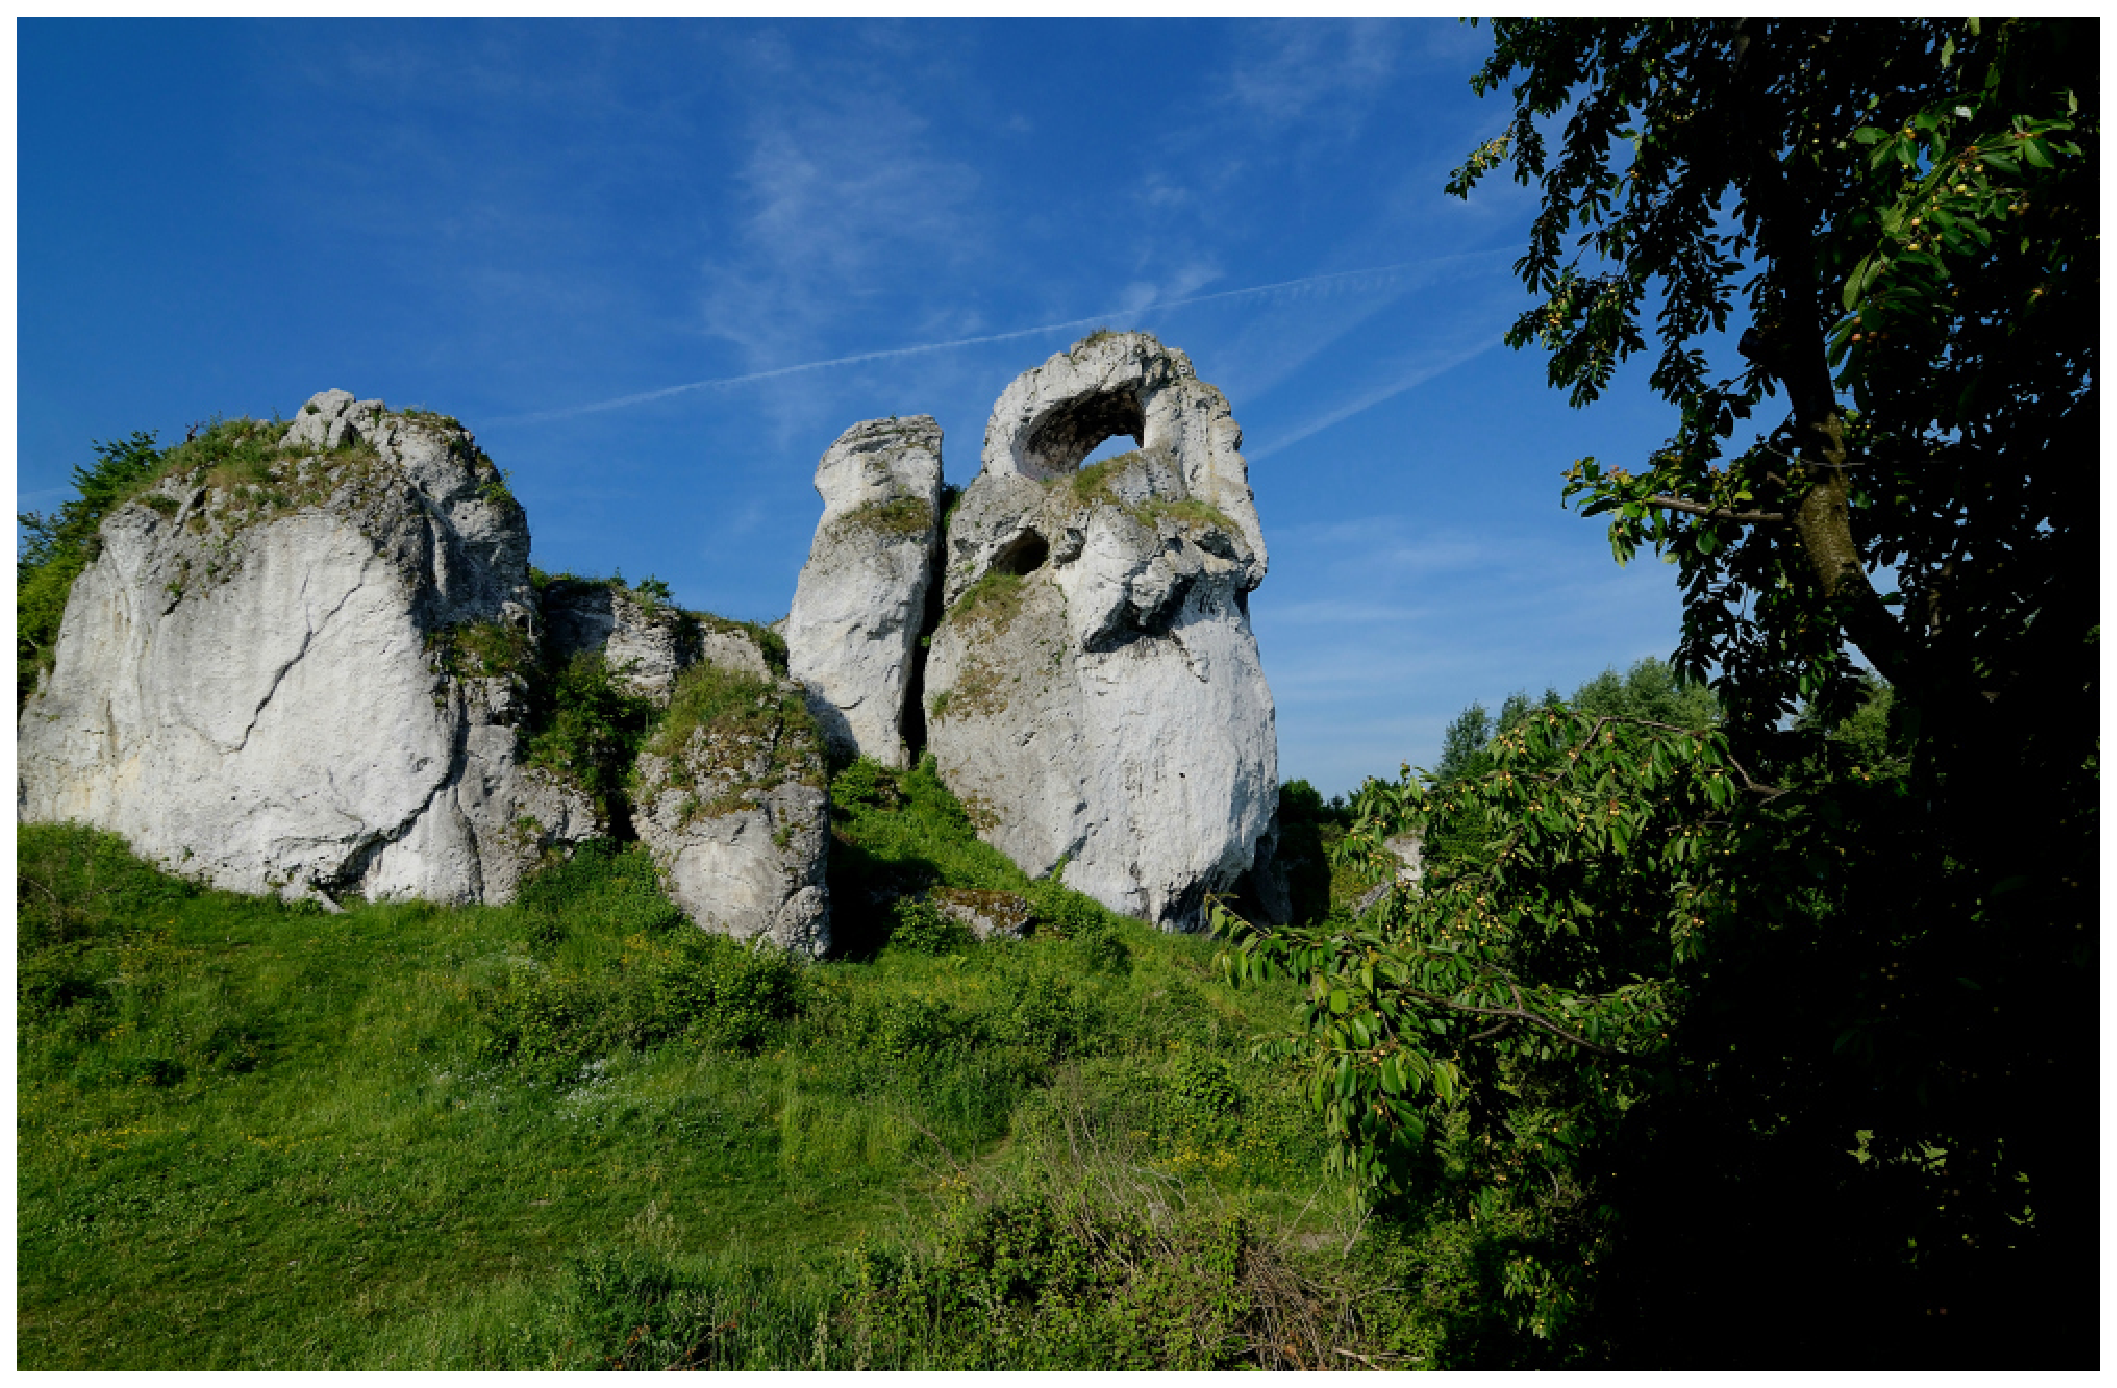
\includegraphics[width=0.9\linewidth]{images/jura-okiennik.eps}
	\end{center}
	\caption{Takie piękne skałki możemy spotkać na Jurze. Główna ściana Okiennika Wielkiego widziana od wschodu (fot. Paweł Wrona)\cite{jura-okiennik}.}
	\label{}
\end{figure}

Jako, że jestem zupełnym amatorem jeśli chodzi o wspinaczkę skałkową, poniżej postaram się przedstawić dwa przykładowe rejony Jury odpowiednie do rozpoczęcia przygody ze wspinaniem \cite{jura-okiennik}. 

\subsubsection{Rzędkowice}
Rzekomo wielu wspinaczu tutaj zaczyna swoją przygodę z Jurą. Jednym z powodów, może być fakt, że początkujący wspinacz znajdzie tutaj ponad 200 linii o wycenie do VI+ włącznie \cite{jura-rzedkowice}. Zdaniem Pawła Wrony z 8academy na początek wspinania w tym rejonie, godnymi uwagi może być skała \textit{Zegarowa} (rysunek \ref{zegarowa}) wraz z trasami \textit{Połupany filarek III} czy \textit{Ostatnią IV+} \cite{jura-rzedkowice}.

\begin{figure}[!htbp]
	\begin{center}
		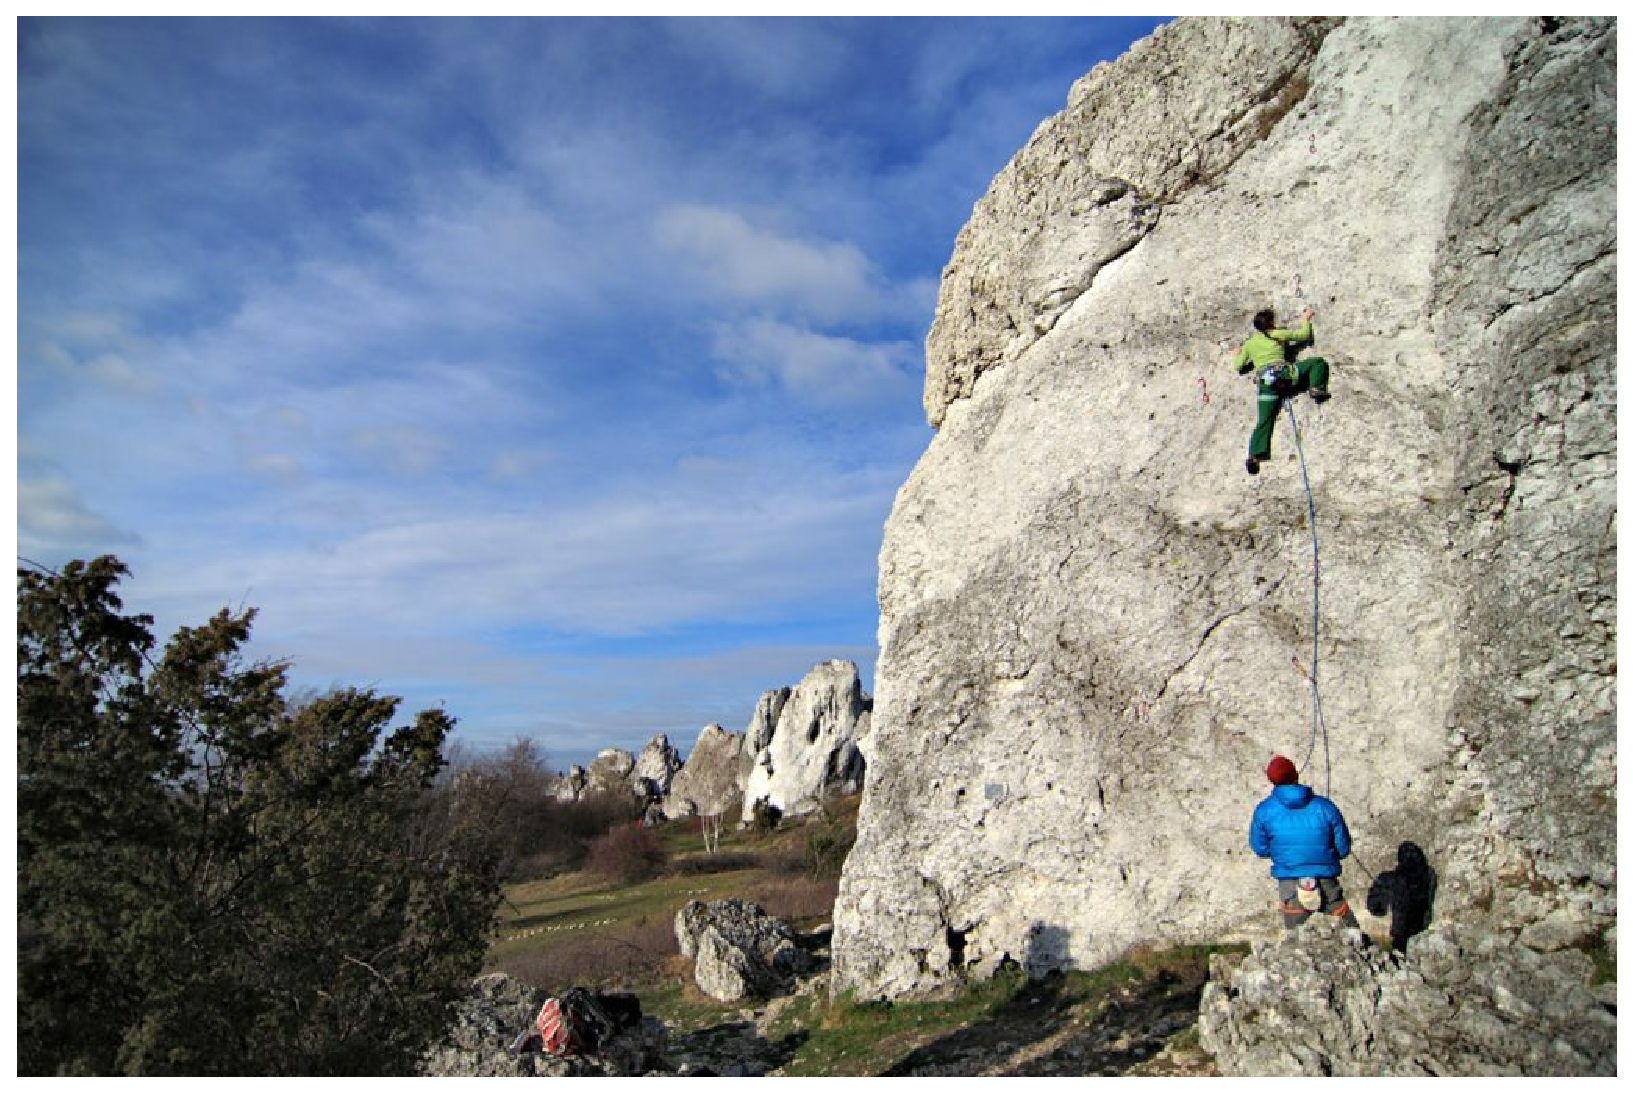
\includegraphics[width=0.9\linewidth]{images/jura-zegarowa.eps}
	\end{center}
	\caption{Wspinanie na Zegarowej, Rzędkowice (fot. Paweł Wrona)\cite{jura-rzedkowice}.}
	\label{zegarowa}
\end{figure}

\subsubsection{Góra Zborów}
Rezerwat Góra Zborów znajduje się w pobliżu miejscowości Podlesice. Znajdziemy tutaj wytyczonych ponad 100 tras wycenionych poniżej VI+ włącznie \cite{topo-gora-zborow}. Początkujący będą mieli zatem z czego wybierać. Ponownie posiłkując się opinią Pawła Wrony, warto na początek rozważyć skałę \textit{Gąsieckiego} z trasami \textit{Dziurki całkiem prawe IV}, \textit{Mały Wachowicz V+} lub \textit{Dziurki VI}. Jeśli chcielibyśmy spróbować czegoś trudniejszego, możemy powspinać się na skale \textit{Młynarz}, gdzie zostały poprowadzone m.in. trasy \textit{Lewy Młynarz VI+} i \textit{Prawy Młynarz VI} \cite{jura-gora-zborow}.

\begin{figure}[!htbp]
	\begin{center}
		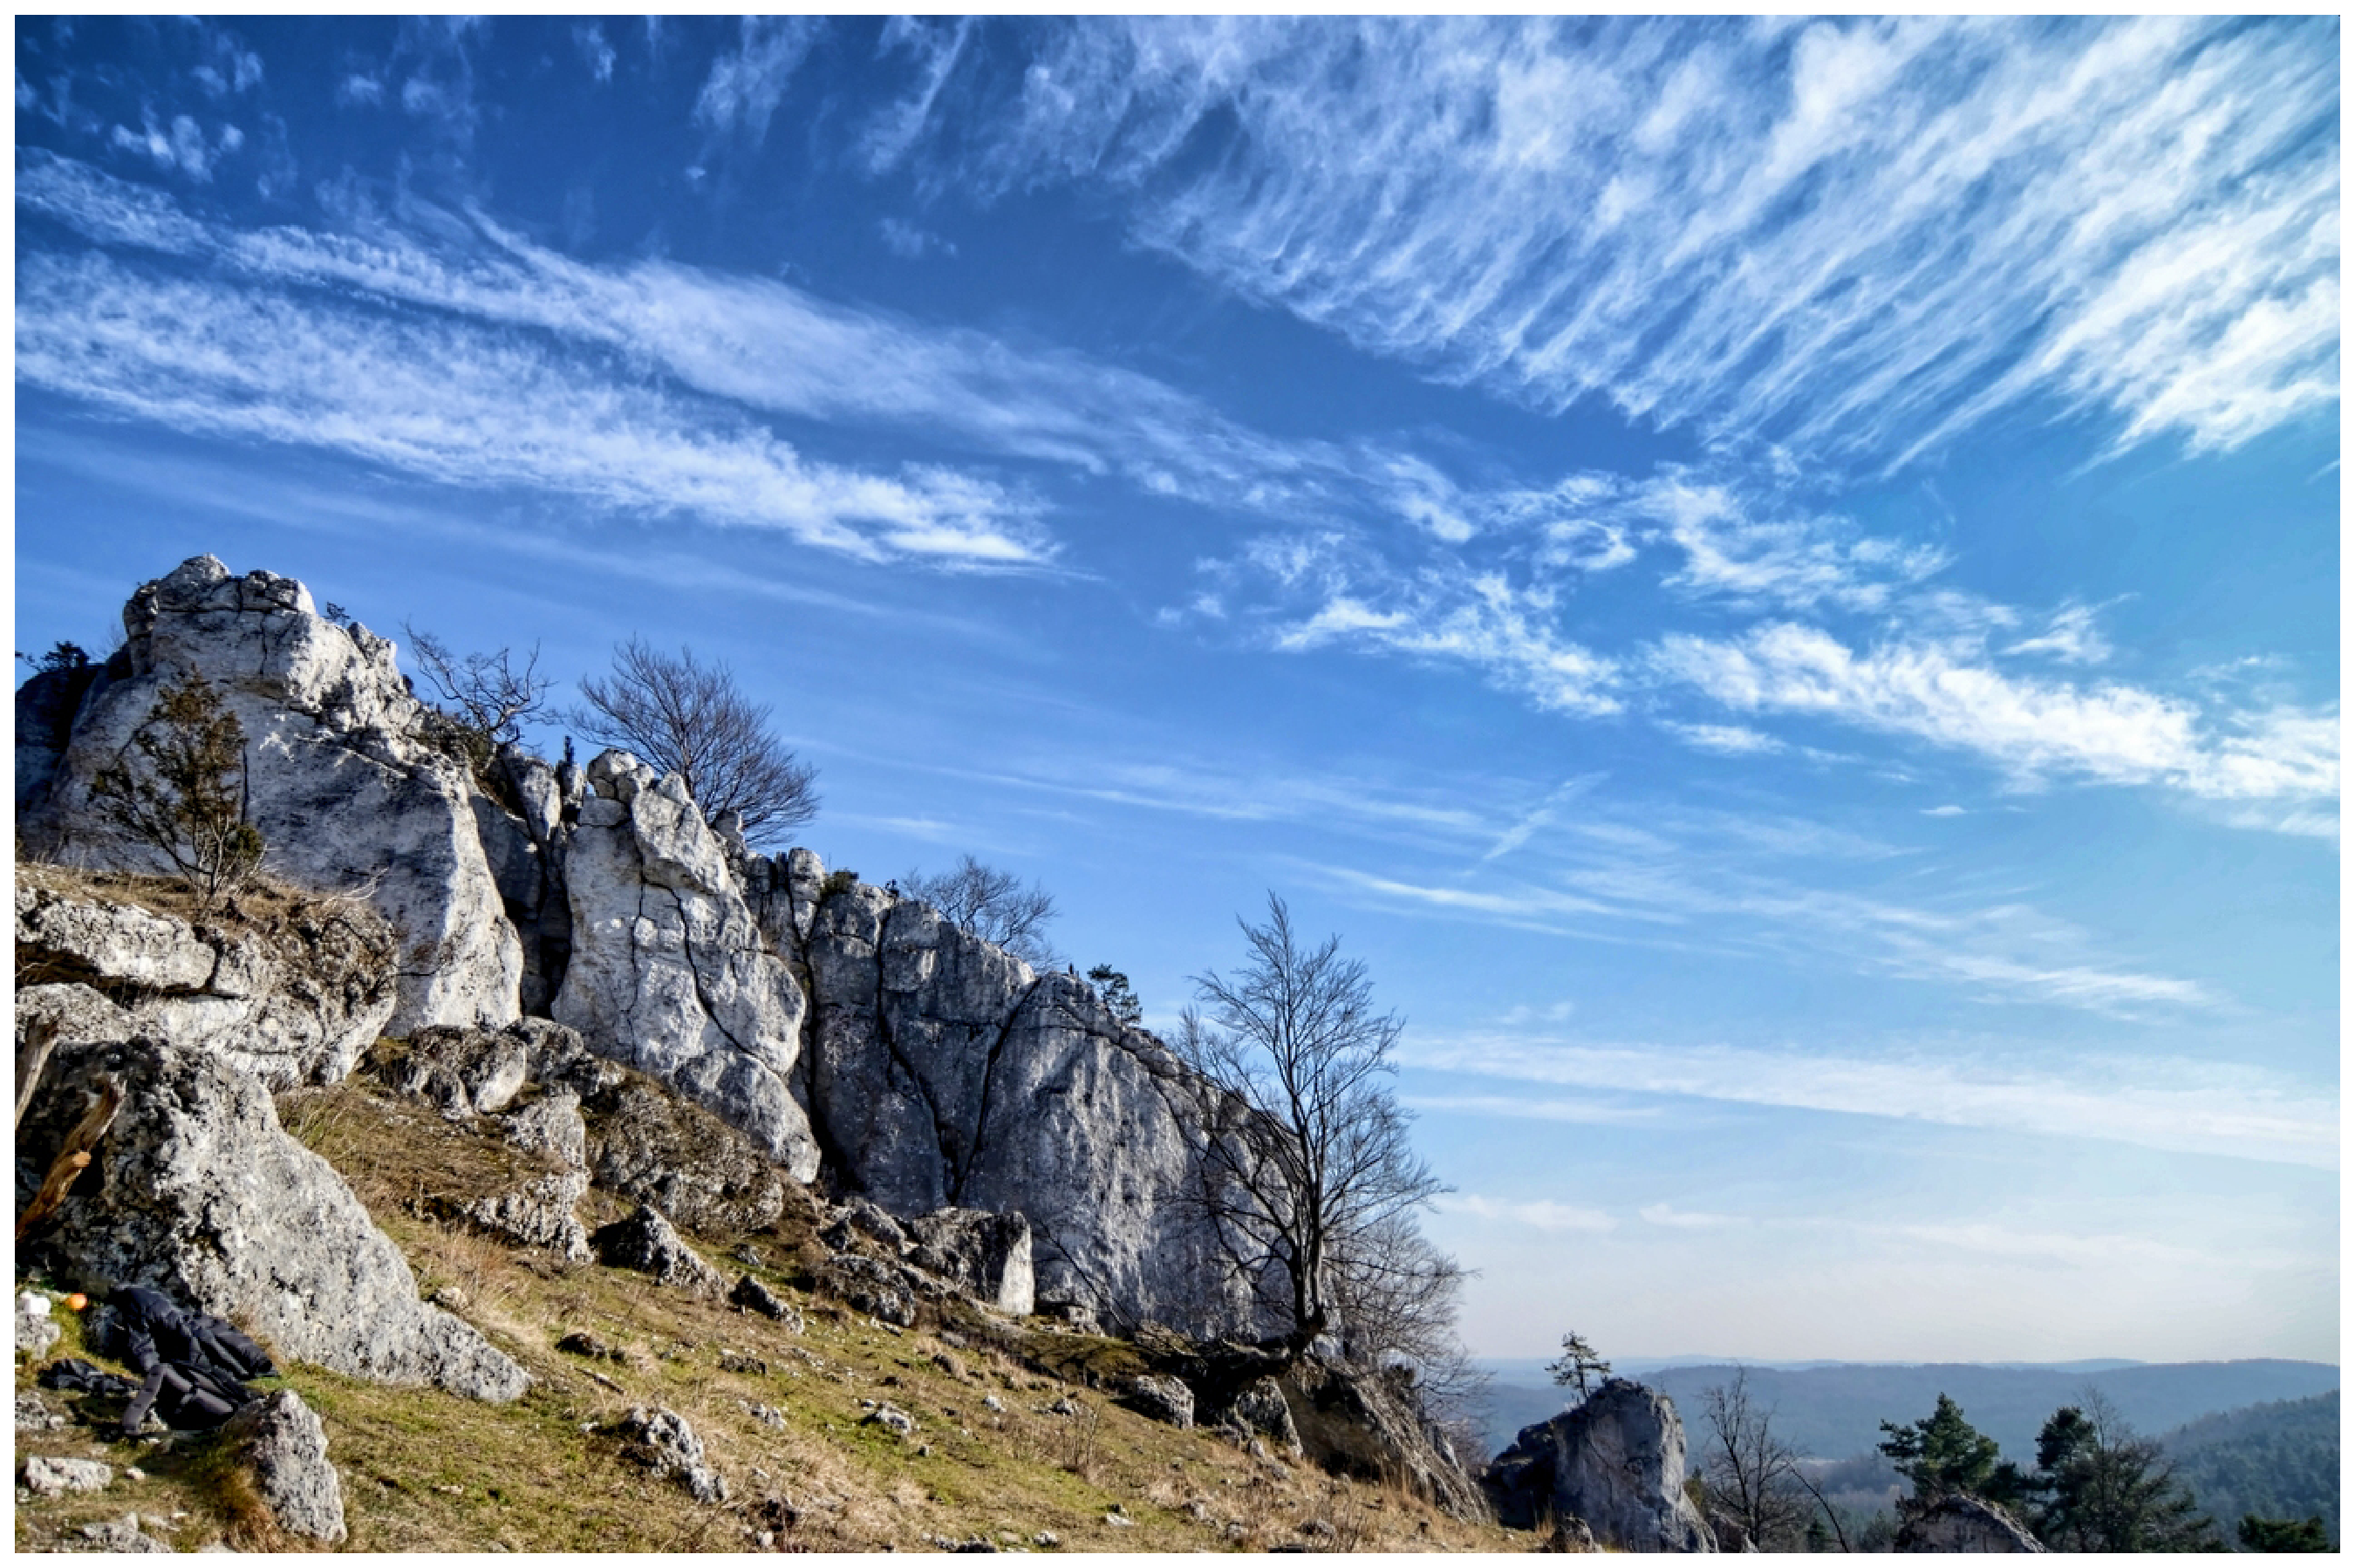
\includegraphics[width=0.9\linewidth]{images/jura-gora-zborow.eps}
	\end{center}
	\caption{Długa grań z widoczną po lewej ścianą \textit{Dziurek} (fot. Paweł Wrona)\cite{jura-gora-zborow}.}
	\label{zborow}
\end{figure}

\begin{figure}[!htbp]
	\begin{center}
		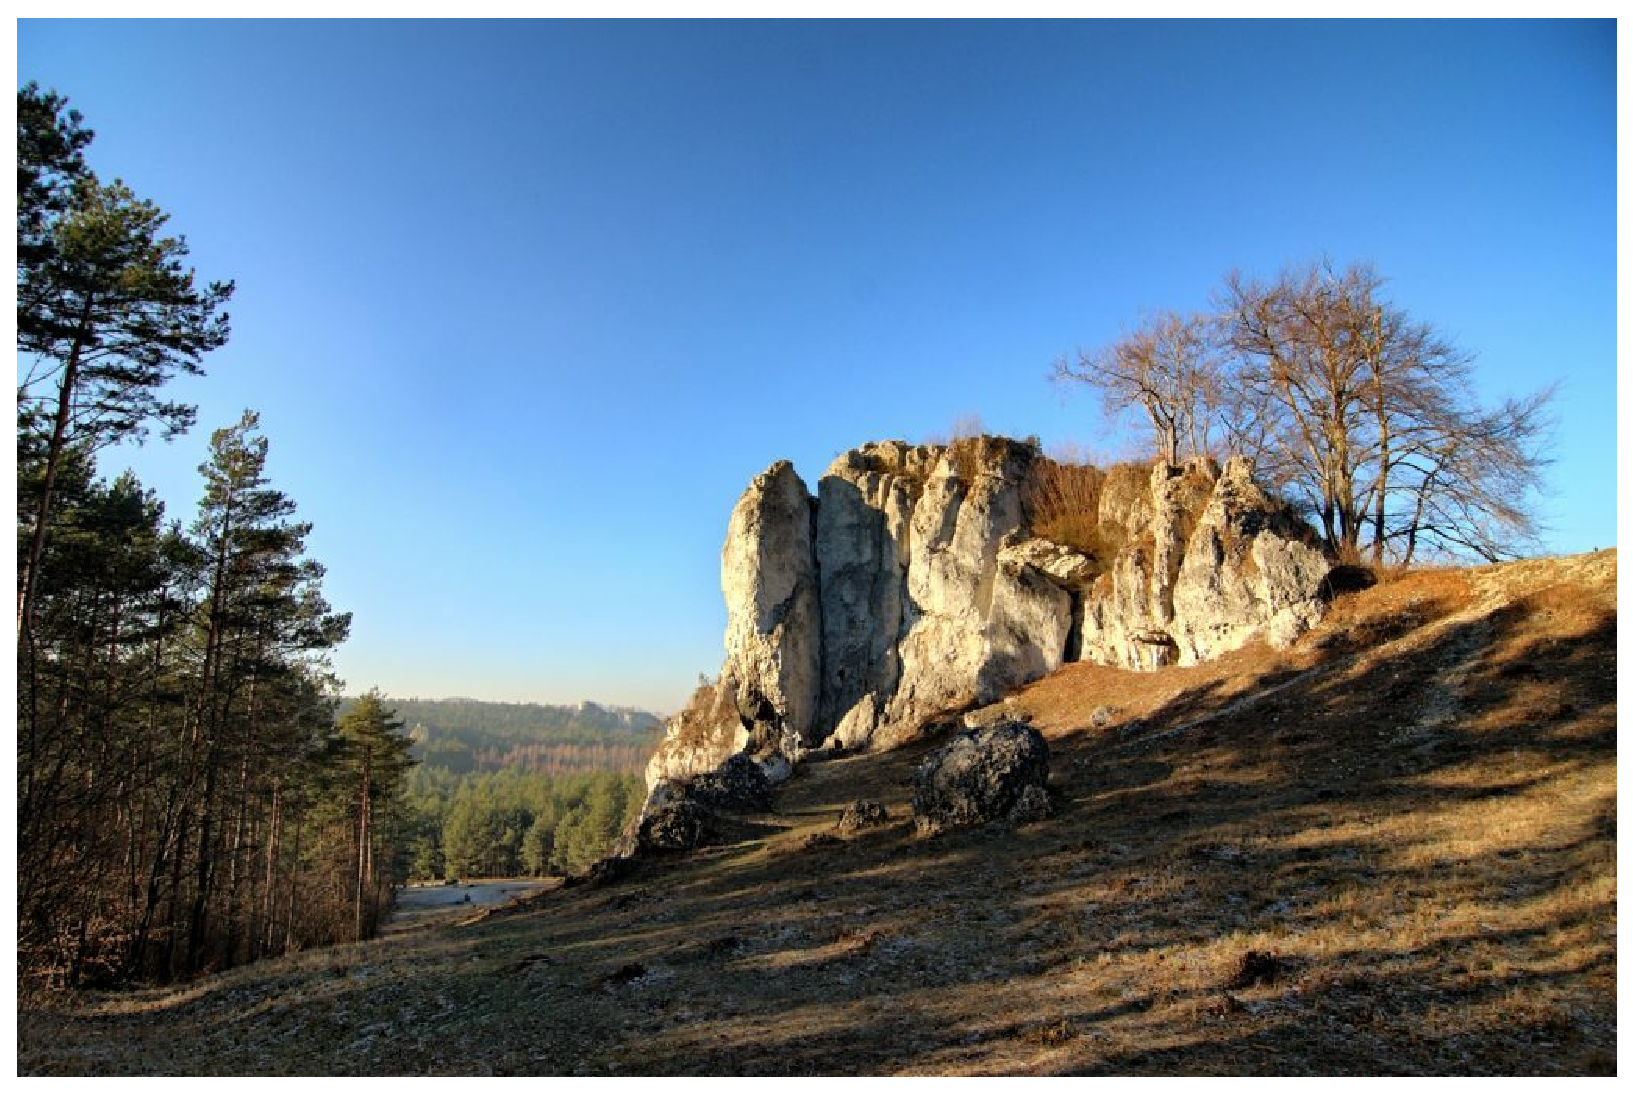
\includegraphics[width=0.9\linewidth]{images/jura-gora-zborow-2.eps}
	\end{center}
	\caption{Okolice Kruka, Góra Zborów (fot. Paweł Wrona)\cite{jura-gora-zborow}.}
	\label{}
\end{figure}

\subsection{Sokoliki}

\subsection{Góry Stołowe}

\nocite{*}
\addcontentsline{toc}{section}{Bibliografia}
\printbibliography

\end{document}
